\documentclass[a4paper, 11pt]{article}
\usepackage[margin=1in]{geometry}
\usepackage[polish]{babel}
\usepackage[T1]{fontenc}
\usepackage[utf8]{inputenc}
\usepackage{hyperref}
\usepackage{array}
\usepackage{amssymb}
\usepackage{amsmath}
\usepackage{listings}
\hypersetup{
    colorlinks,
    citecolor=black,
    filecolor=black,
    linkcolor=black,
    urlcolor=black
}
\usepackage{graphicx}

\usepackage{tikz}
\usetikzlibrary{fit,arrows,matrix,positioning, calc, shapes.gates.logic.IEC, shapes.gates.logic.US,arrows,arrows.meta}
\tikzstyle{branch}=[fill,shape=circle,minimum size=3pt,inner sep=0pt]

\definecolor{codegreen}{rgb}{0,0.6,0}
\definecolor{codegray}{rgb}{0.5,0.5,0.5}
\definecolor{codepurple}{rgb}{0.58,0,0.82}
\definecolor{backcolour}{rgb}{0.95,0.95,0.92}

\lstdefinestyle{mystyle}{
    backgroundcolor=\color{backcolour},   
    commentstyle=\color{codegreen},
    keywordstyle=\color{magenta},
    numberstyle=\tiny\color{codegray},
    stringstyle=\color{codepurple},
    basicstyle=\ttfamily\footnotesize,
    breakatwhitespace=false,         
    breaklines=true,                 
    captionpos=b,                    
    keepspaces=true,                 
    numbers=left,                    
    numbersep=5pt,                  
    showspaces=false,                
    showstringspaces=false,
    showtabs=false,                  
    tabsize=4
}

\lstset{style=mystyle}

\title{%
        \vspace{-2cm}
       \large Sprawozdanie Laboratorium PTC \\
       \huge Synteza wyższego poziomu.}

\author{Stanisław Fiedler 160250, L1}
\date{LAB 7, 20 stycznia 2025}

\begin{document}

\maketitle
%\tableofcontents

\section{Zadanie 4}\label{sec:zadanie_} % (fold)

\begin{description}
	\item[a)] Narysuj diagram maszyny algorytmicznej realizującej automat z poprzedniego zadania.
	\item[b)] Korzystając z programu Deeds FSM zasymuluj działanie maszyny algorytmicznej.
\end{description}

\subsection{Diagram ASM}\label{sub:diagram_asm} % (fold)
\begin{center}
	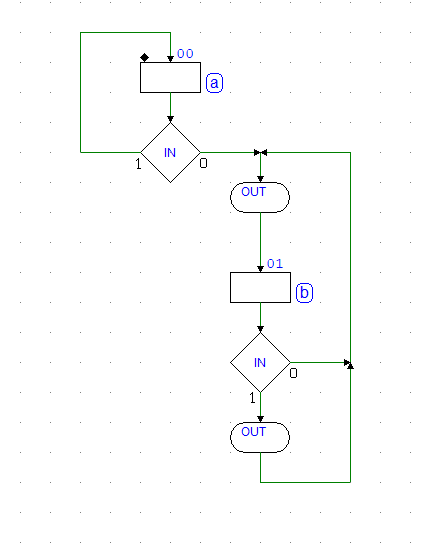
\includegraphics[scale=0.6]{images/asm_4.png}
\end{center}
% subsection Diagram ASM (end)

\subsection{Symulacja}\label{sub:symulacja} % (fold)
\begin{center}
	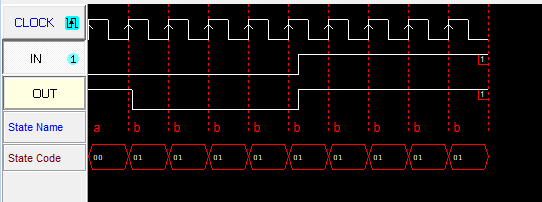
\includegraphics[scale=0.7]{images/4_sym_0.png}
	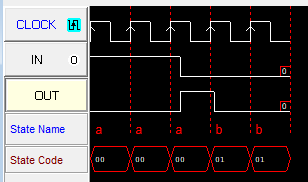
\includegraphics[scale=0.8]{images/4_sym_1.png}
\end{center}
% subsection Symulacja (end)

% section Zadanie 4 (end)

\section{Zadanie 7}\label{sec:zadanie_} % (fold)
Licznik z zadania 6 zrealizowano wykorzystując przerzutniki D. Ogólną strukturę układu pokazano na rysunku 2.
Zakładając, że A oznacza wyjście najbardziej znaczącego przerzutnika, a E jest wejściem
wybierającym kierunek zliczania (0 – w górę, 1- w dół) wyznacz funkcje wzbudzeń przerzutników
A, B, C, D (bez minimalizacji).
\[
	A = \bar{A}\bar{B}\bar{C}D\bar{E} + \bar{A}B\bar{C}\bar{D}E
\]
\[
	B = A\bar{B}\bar{C}\bar{D}\bar{E} + \bar{A}\bar{B}C\bar{D}E
\]
\[
	C = \bar{A}B\bar{C}\bar{D}\bar{E} + \bar{A}\bar{B}\bar{C}DE
\]
\[
    D = \bar{A}\bar{B}C\bar{D}\bar{E} + A\bar{B}\bar{C}\bar{D}E
\]
% section Zadanie 7 (end)

\end{document}
